\chapter{Razvijeni sustav za detekciju plagijata te utvrđivanje autorstva izvornih kodova}

Razvijeni sustav za detekciju plagijata sastoji se od dvije komponente čiji su  algoritmi opisani u prethodnim poglavljima. Ovdje ukratko opisujemo njihove implementacije te arhitekturu cijelog sustava. Prva komponenta razvijenog sustava je utvrđivanje autorstva izvornog koda te je ona razdvojena u poseban projekt nazvan $Bee$. Ovo omogućuje lakši razvoj algoritama strojnog učenja s kojim utvrđujemo autorstvo te nam daje veću fleksibilnost za korištenje te komponente izvan konteksta detekcije plagijata. $Bee$ je dizajniran kao skripta komandne linije kojoj se predaju skup za treniranje i skup za testiranje te koja vraća točnost naučenog klasifikatora jer nam taj način nudi lako isprobavanje raznih konfiguracija i skupova izvornih kodova. $Turtle$ je druga i ujedno glavna komponenta sustava koja određuje sličnosti izvornih kodova te nudi korisnicima web sučelje za pristup algoritmima detekcije plagijata. Korisnici mogu vidjeti sortirane parove izvornih kodova te njihove pripadne sličnosti nakon što uploadaju željenu datoteku s izvornim kodovima. Sustav nudi i detaljniji uvid u parove izvornih kodova i to tako da jednakim bojama boja slične dijelove izvornih kodova. Arhitektura cijelog sustava detaljnije je opisana je u poglavlju \ref{sec:architecture}. Sustav se također spaja na sustav $Bee$ te je moguće trenirati klasifikator i predviđati autore kroz njegove sučelje. 
\\

	Ovaj sustav je prvi sustav koji nudi korisnicima detekciju plagijata kroz dva različita načina te je ovo veliko unaprijeđenje na sve dosadašnje sustave za detekciju plagijata izvornih kodova. $Turtle$, a također i $Bee$ trenutno podržavaju samo programski jezik $C++$ iako je u implementacijama obje komponente ostavljena mogućnost lakog dodavanja novih jezika, ali to je ostavljeno za budući rad. Ovo poglavlje opisuje i korisničko sučelje sustava $Turtle$.


\section{Arhitektura sustava} \label{sec:architecture}
Spomenuto je da je $Bee$ dizajniran kao skripta komandne linije te je bilo potrebno nekako ga spojiti s drugom komponentom. To je napravljeno tako da je napisan jednostavan web server koji nudi nekoliko API endpoint-a na korištenje ostalim aplikacijama. Ti endpoint-i izvršavaju metode poput učenja klasifikatora ili predviđanja autora. Ovakav dizajn nam nudi mogućnost korištenja utvrđivanja autorstva i izvan konteksta sustava $Turtle$, a njemu nudi lagano povezivanje. Klijentski kod $Turtle$ aplikacije se kada to korisnik zatraži spaja na API endpoint-e ponuđene iz $Bee$ te ispisuje vraćene podatke korisniku na ekran. Sve ovo detaljnije možemo vidjeti na slici \ref{fig:architecture}.

\begin{figure}[H]
	\centering
	\fbox{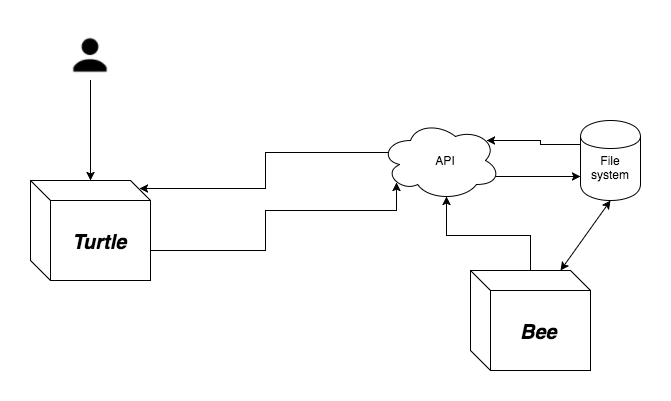
\includegraphics[width=0.9\textwidth,keepaspectratio]{fig/turtle_architecture.png}}
	\caption{Arhitektura razvijenog sustava}
	\label{fig:architecture}
\end{figure}

\newpage
\section{Korisničko sučelje}

U ovom potpoglavlju opisano je korisničko sučelje sustava $Turtle$ kroz nekoliko slika.


\begin{figure}[H]
	\centering
	\fbox{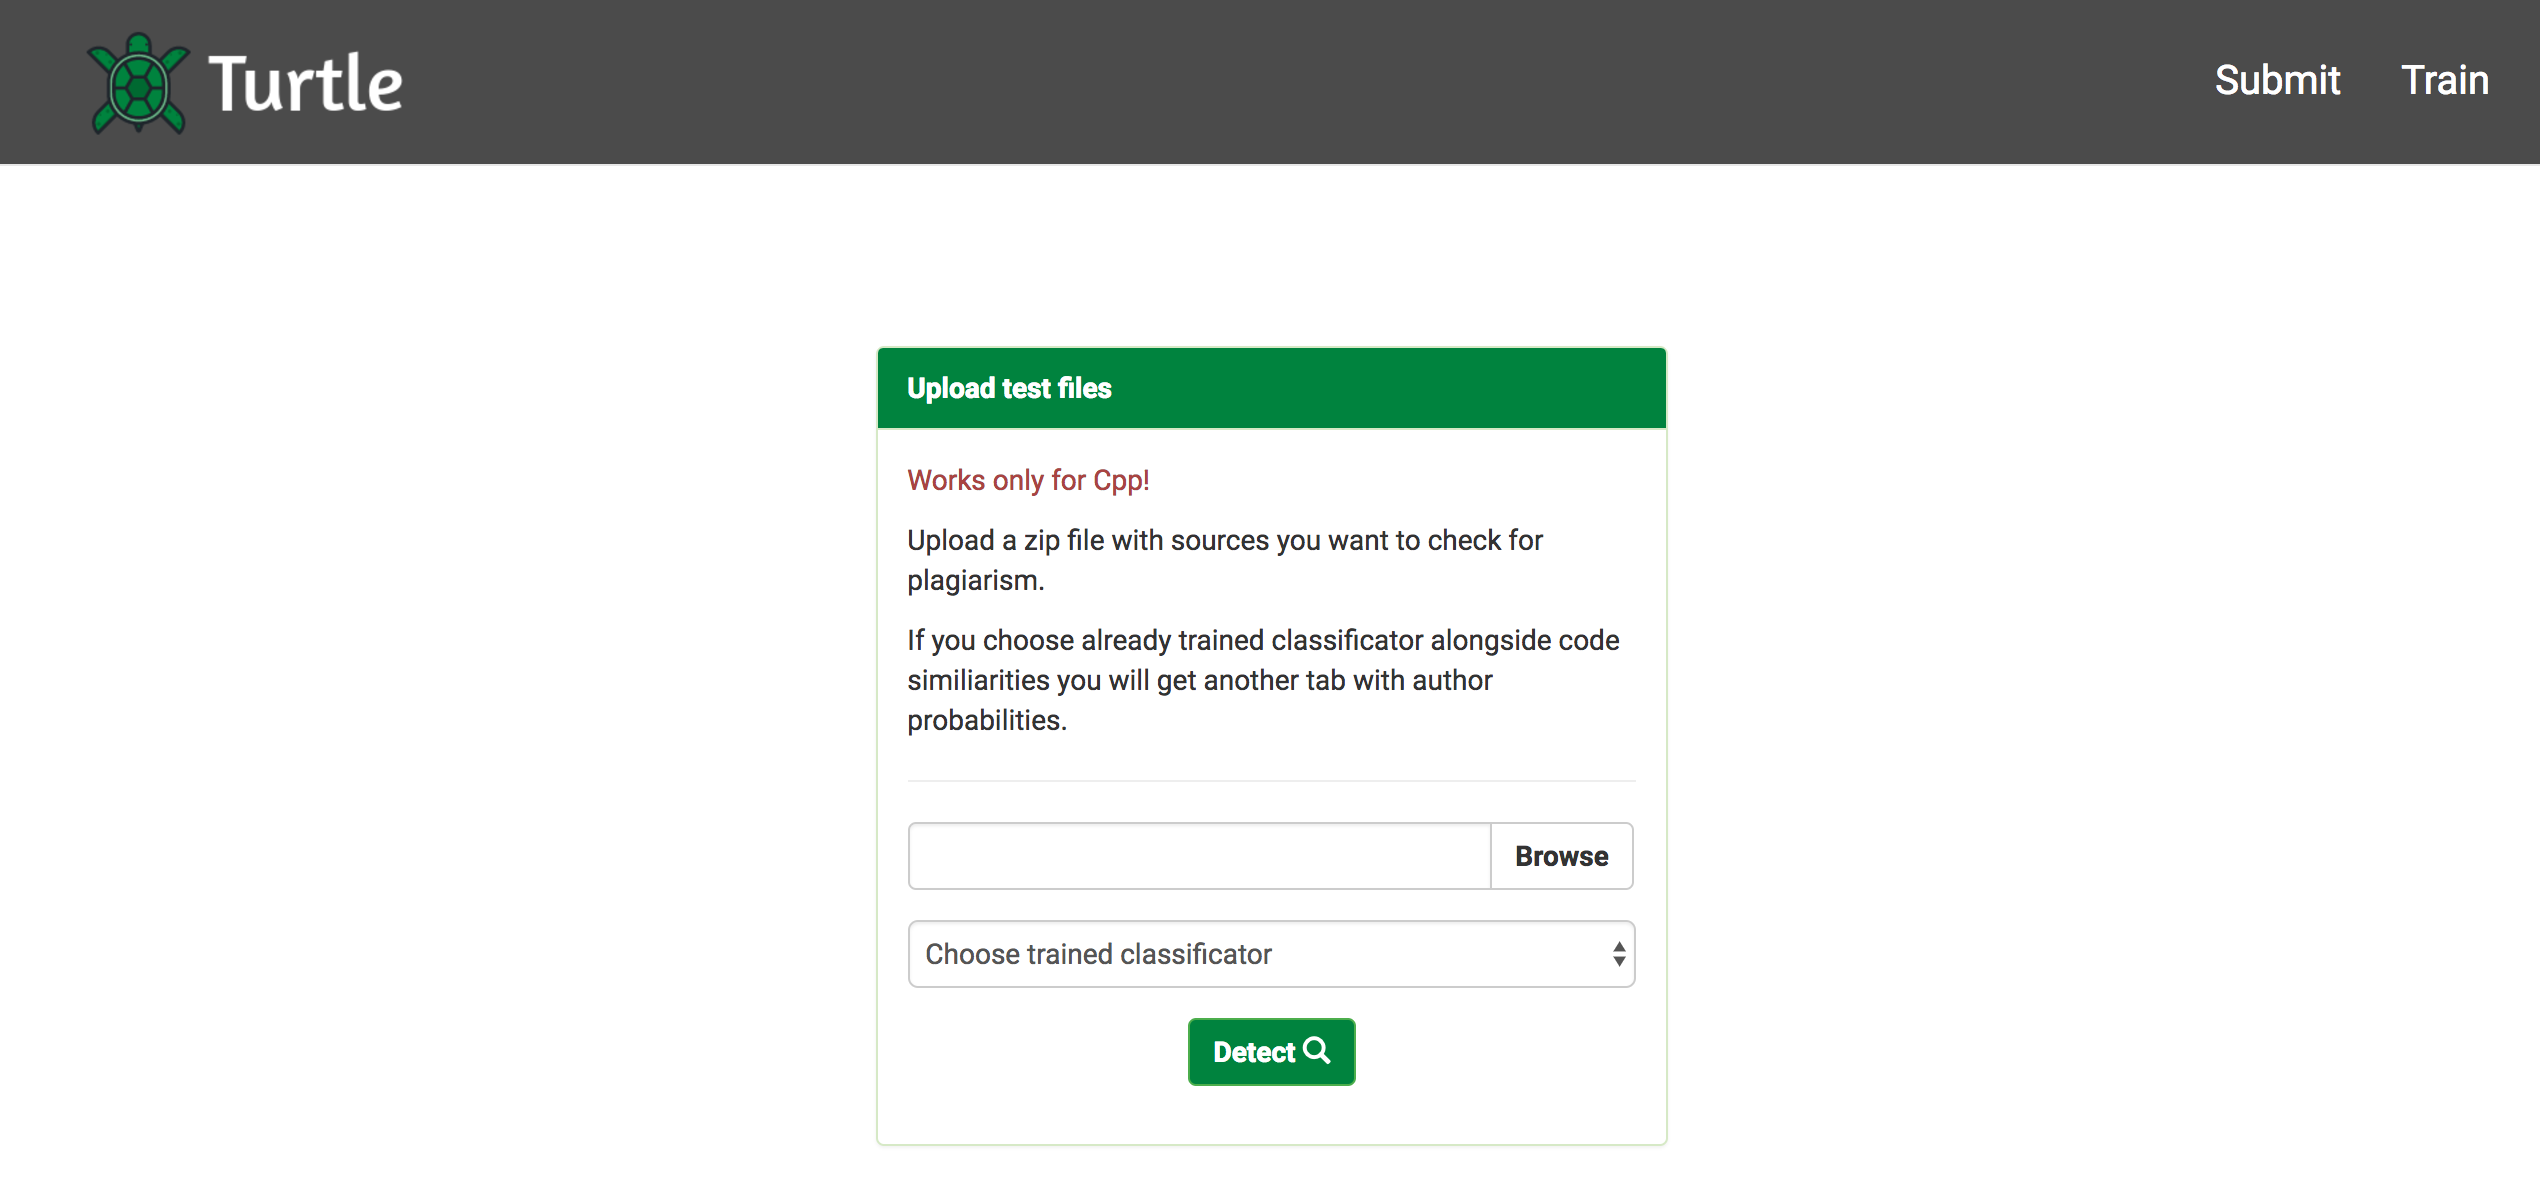
\includegraphics[width=0.9\textwidth,keepaspectratio]{fig/submit.png}}
	\caption{Početna stranica, ovdje uploadamo zip datoteku koju želimo provjeriti, također možemo izabrati unaprijed trenirani klasifikator kako bi mogli dobili i najvjerojatnije autore svakog koda.}
\end{figure}

\begin{figure}[H]
	\centering
	\fbox{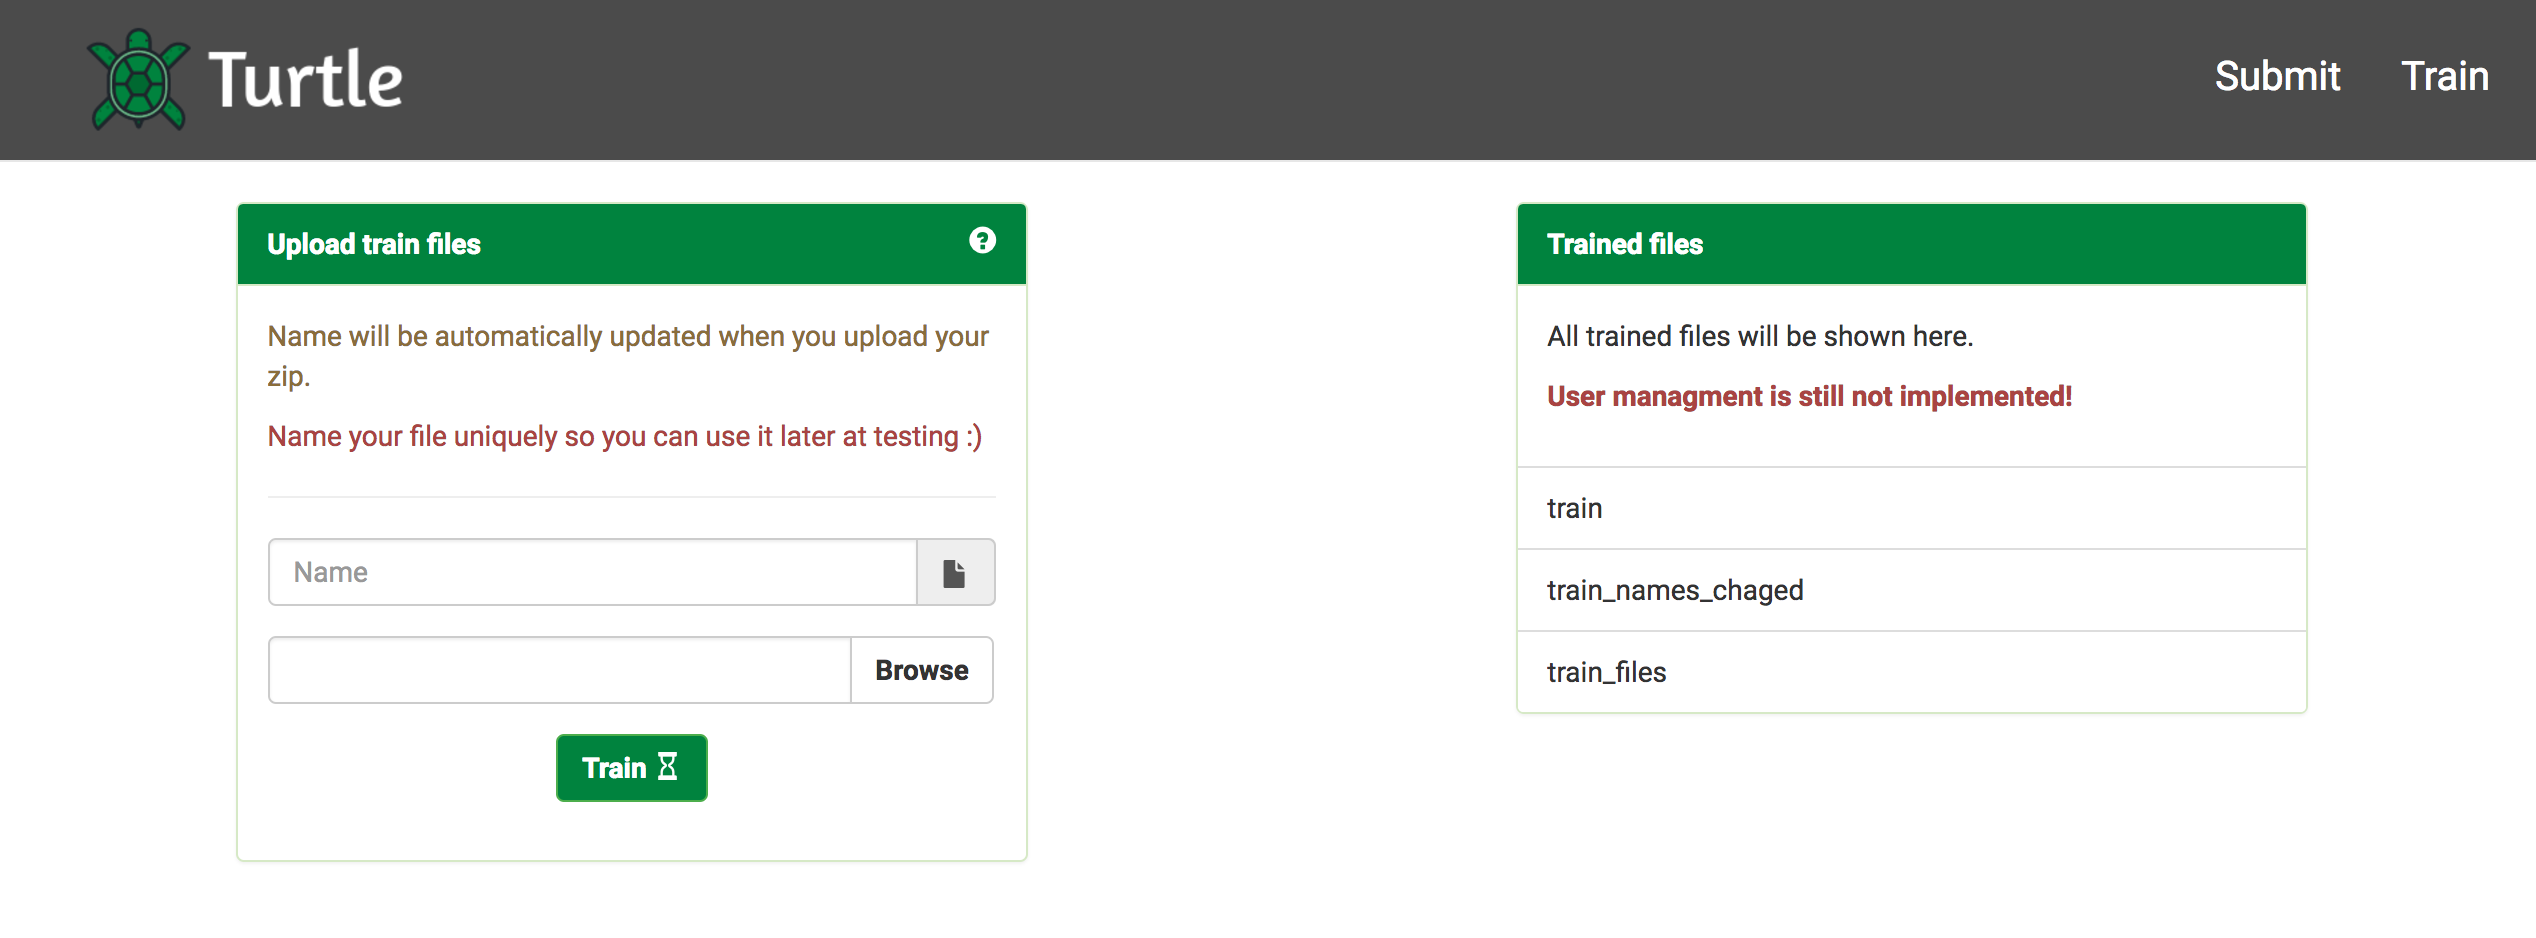
\includegraphics[width=0.9\textwidth,keepaspectratio]{fig/train.png}}
	\caption{Stranica za treniranje klasifikatora, uploada se zip datoteka te nakon što je učenje završeno naučeni klasifikator se pojavi u listi desno.}
\end{figure}

\begin{figure}[H]
	\centering
	\fbox{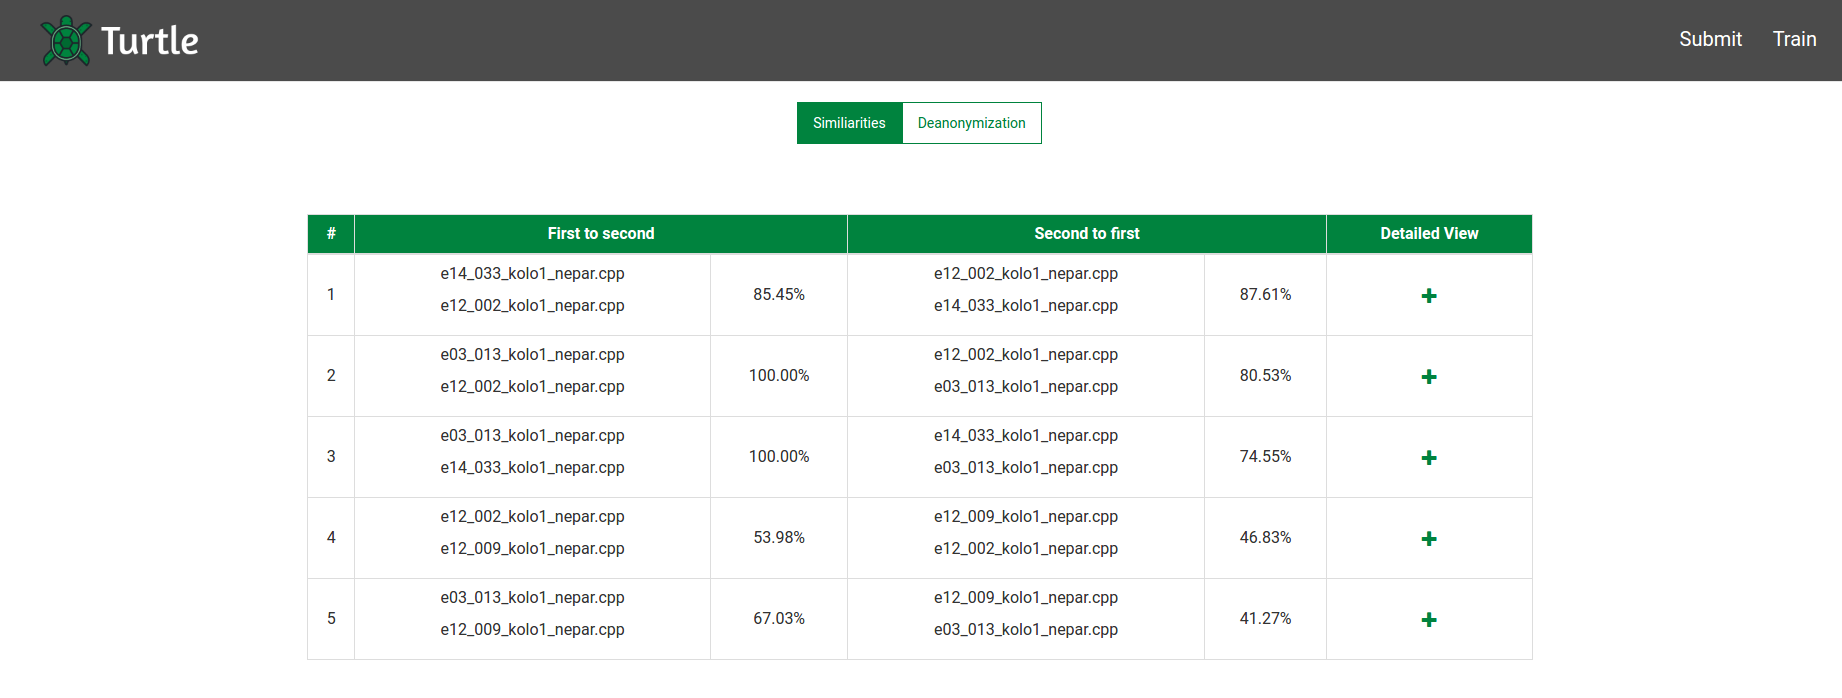
\includegraphics[width=0.9\textwidth,keepaspectratio]{fig/pairs.png}}
	\caption{Nakon što sustav pronađe sve sličnosti ispiše nam ih u tablicu sortirane od najveće do najmanje sličnosti.}
\end{figure}

\begin{figure}[H]
	\centering
	\fbox{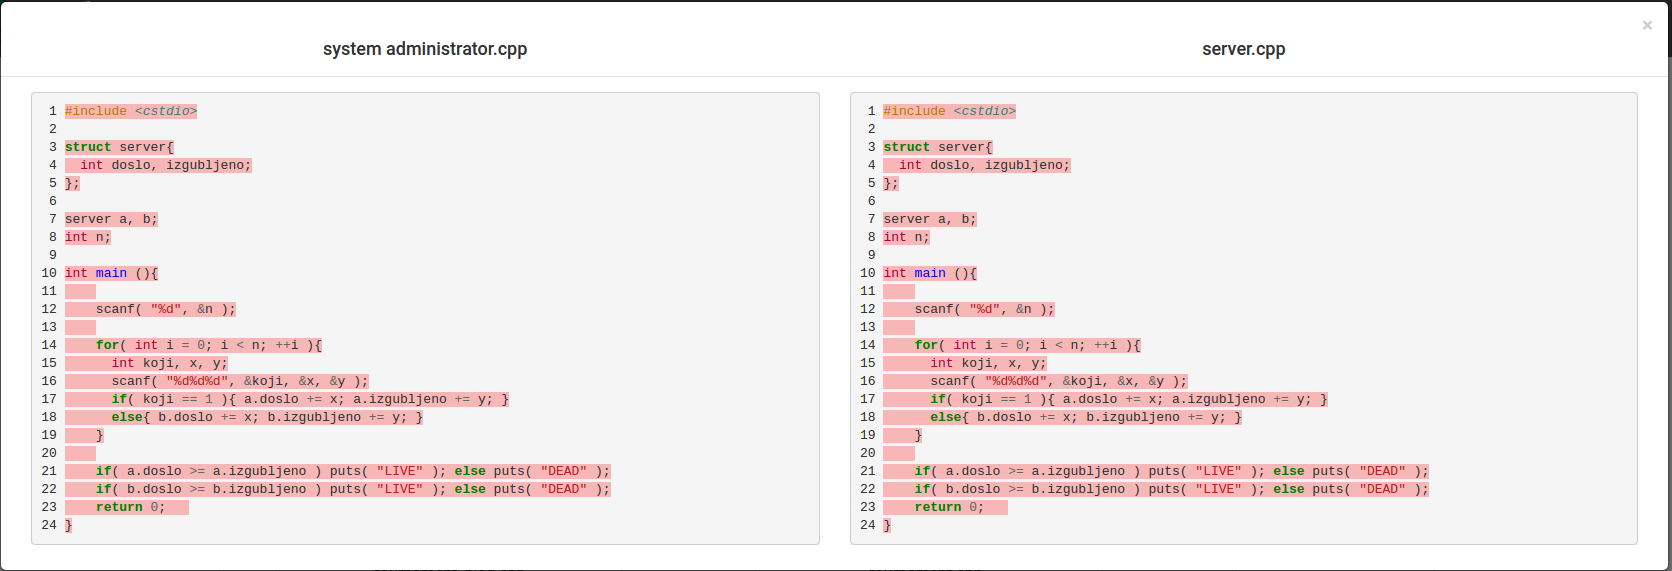
\includegraphics[width=0.9\textwidth,keepaspectratio]{fig/colors.png}}
	\caption{Ako kliknemo na više detalja koji postoji za svaki par izvornih kodova dobijemo ovakav prozor gdje su obojeni dijelovi koda koji su slični i što nam uvelike olakšava detekciju plagijata.}
\end{figure}

\begin{figure}[H]
	\centering
	\fbox{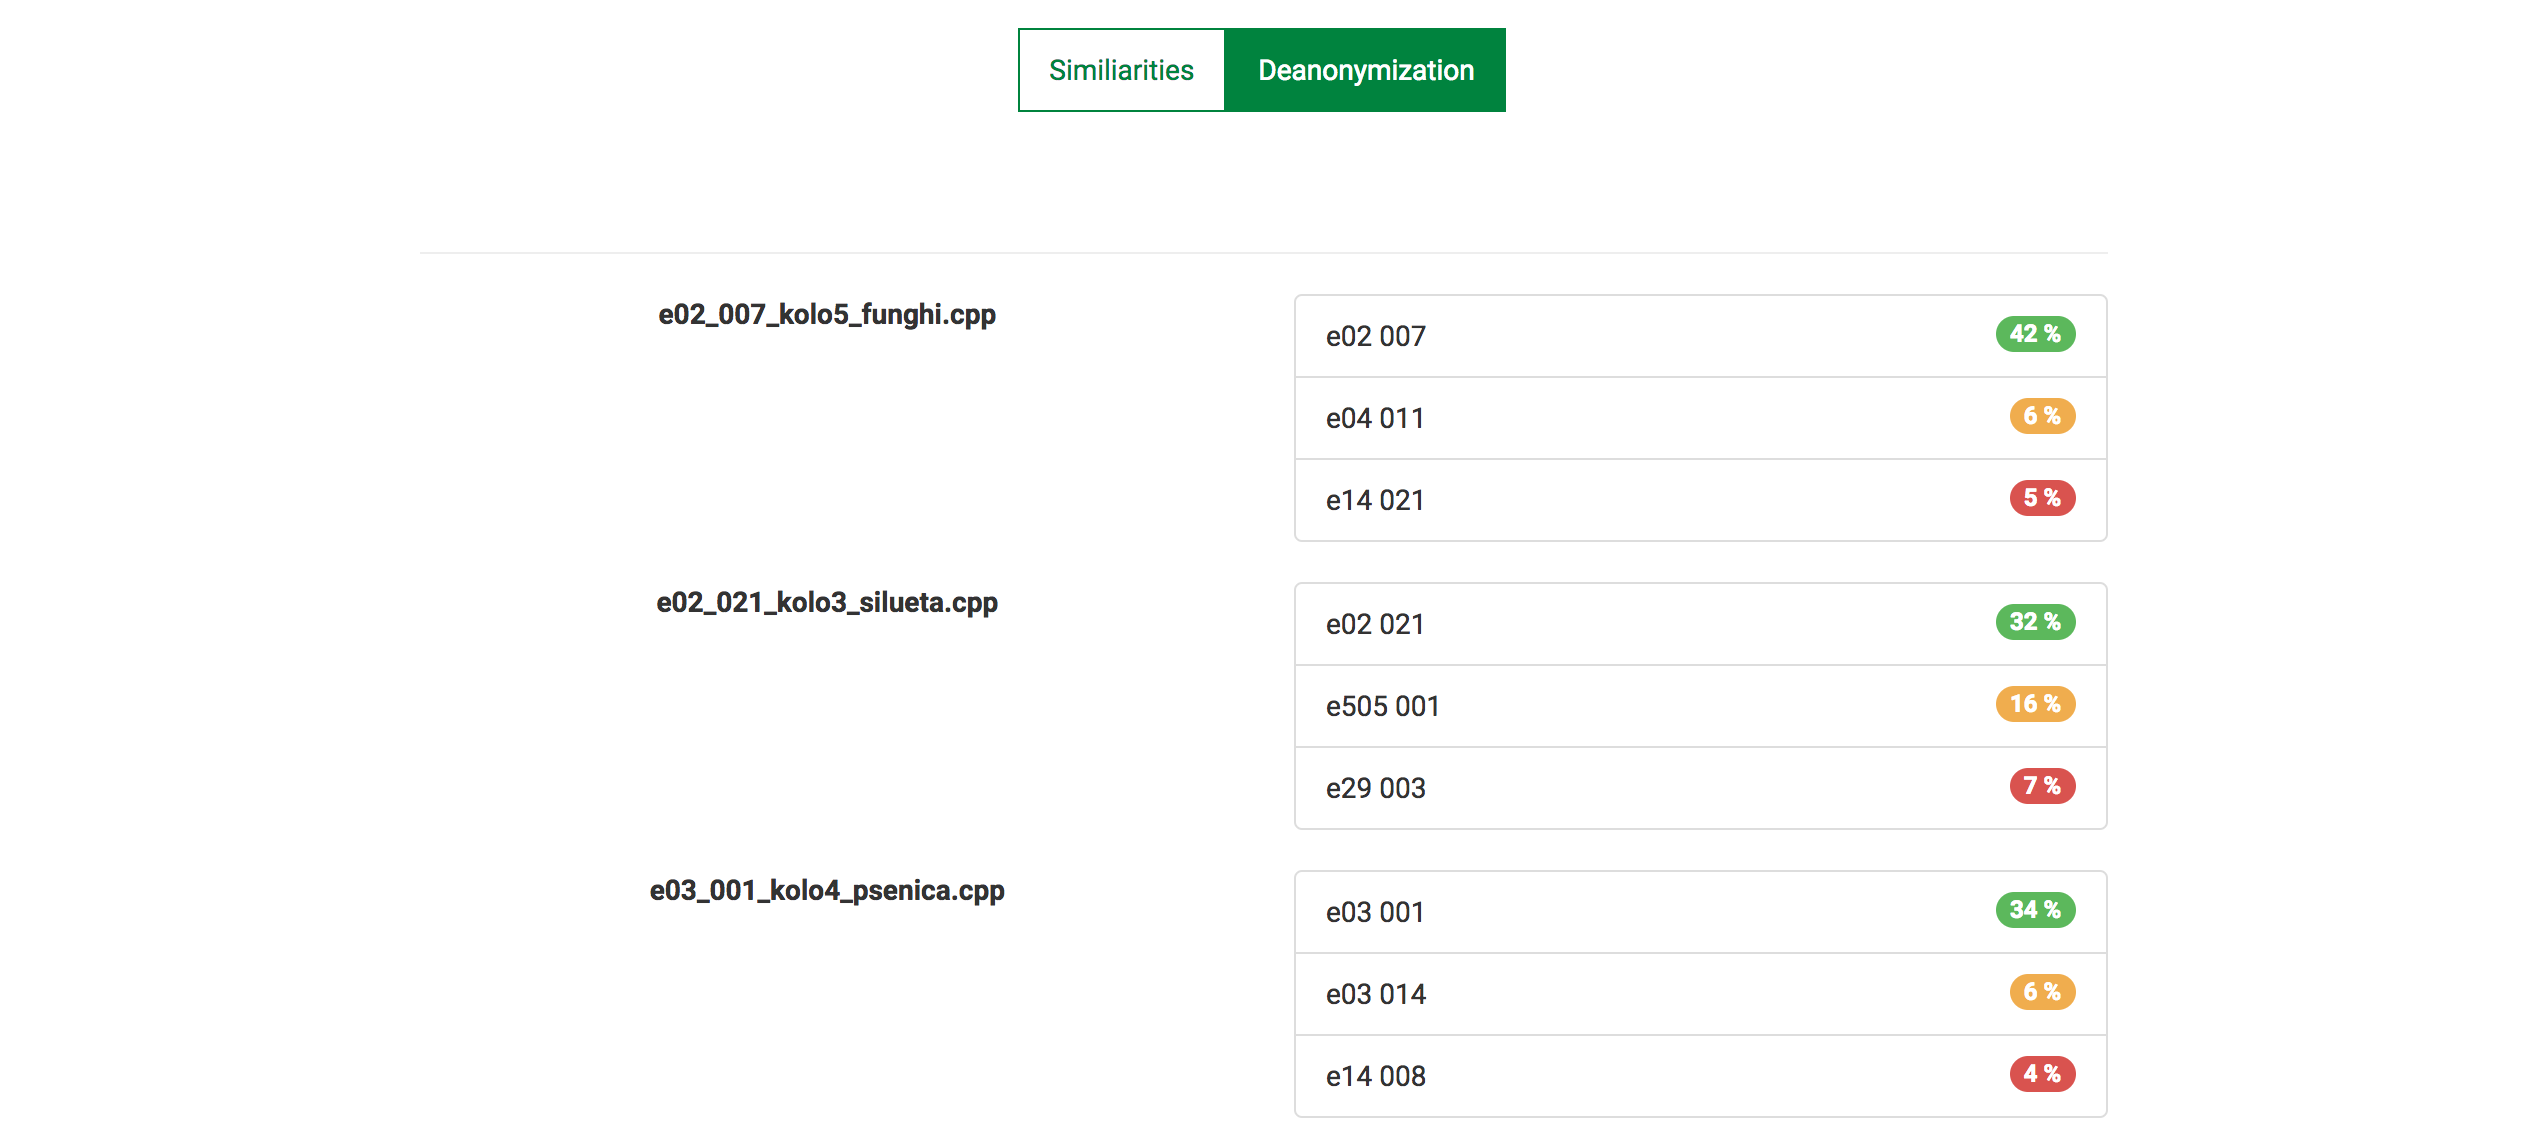
\includegraphics[width=0.9\textwidth,keepaspectratio]{fig/authors.png}}
	\caption{Ako smo uz detekciju plagijata odredili da želimo i provjeriti tko bi mogli biti autori naših kodova na tabu \textit{Deanonymization} dobijemo za svaki izvorni kod listu od 3 najvjerojatnija autora.}
\end{figure}


\section{Implementacijski detalji}

\subsection{Turtle}
Za implementaciju korišten je programski jezik \textit{Python 2.7.} Web server napisan je u random okviru \textit{Flask} \footnote{http://flask.pocoo.org/}. Klijentski dio aplikacije implementiran je u \textit{ReactJS} \footnote{https://facebook.github.io/react/} frameworku kako bi korisnici imali što bolji doživljaj korištenja aplikacije te zbog asinkronog dohvata podataka.

\subsection{Bee}

\renewcommand{\footnotesize}{\fontsize{8pt}{10pt}\selectfont}

Za implementaciju korišten je programski jezik \textit{Python 2.7} te njegova biblioteka \textit{scikit-learn} \footnote{\url{http://scikit-learn.org/stable/}} koja nudi pristup mnogim algoritmima strojnog učenja na vrlo jednostavan način. Za implementaciju slučajne šume korištena je  klasa \textit{RandomForestClassifier} \footnote{\url{http://scikit-learn.org/stable/modules/generated/sklearn.ensemble.RandomForestClassifier.html}}. Selekcija značajki uzajamnim sadržajem informacije implementirana je pomoću klase \textit{ExtraTreeClassifier} \footnote{\url{http://scikit-learn.org/stable/modules/generated/sklearn.ensemble.ExtraTreesClassifier.html}} koji omogućava biranje idućih čvorova uzajamnim sadržajem informacije (parametar "criterion") te nam nakon učenja omogućava pristup najbitnijim značajkama. Selekcija značajki iznosom varijance implementirana je korištenjem  klase \textit{VarianceThreshold} \footnote{\url{http://scikit-learn.org/stable/modules/generated/sklearn.feature_selection.VarianceThreshold.html}}.
Web dio komponente napisan je u radnom okviru \textit{Flask}.
